\section{EdgeFace: Mô hình nhận diện khuôn mặt hiệu quả cho các thiết bị biên}
\label{sec:edgeface-lessons}

% Giới thiệu ngắn gọn về EdgeFace

\subsection{Mô tả mô hình EdgeNext}

\subsubsection{Giới thiệu về EdgeNext}

EdgeNext là một mô hình mạng nơ-ron thị giác lai (hybrid) được thiết kế đặc biệt dành cho các thiết bị biên (edge devices) với mục tiêu đạt được \textbf{độ chính xác cao} trong khi \textbf{giữ số lượng tham số và chi phí tính toán ở mức tối thiểu} \cite{maaz2022edgenext}. Được giới thiệu trong bài báo ``EdgeNext: Efficiently Amalgamated CNN-Transformer Architecture for Mobile Vision Applications'' (arXiv:2206.10589), EdgeNext kết hợp ưu điểm của \textbf{mạng tích chập (CNN)} -- mạnh về trích xuất đặc trưng cục bộ -- và \textbf{Vision Transformer (ViT)} -- hiệu quả trong việc mã hóa tương tác toàn cục -- nhằm tạo ra một kiến trúc \textbf{tinh gọn, nhanh và phù hợp triển khai thực tế}.

Mô hình được phát triển nhằm giải quyết hai hạn chế chính của các kiến trúc hiện hành:
\begin{itemize}
    \item \textbf{CNN thuần túy} thiếu khả năng tương tác toàn cục giữa các vùng không gian xa nhau.
    \item \textbf{Vision Transformer} tuy mạnh về ngữ cảnh toàn cục nhưng có độ phức tạp tính toán bậc hai $O(N^2)$ (với $N$ là số token), dẫn đến chi phí cao, không phù hợp với thiết bị có tài nguyên hạn chế như điện thoại thông minh hoặc camera giám sát.
\end{itemize}

EdgeNext được thiết kế với các biến thể nhỏ gọn (XXS, XS, S), chỉ từ \textbf{1.3 triệu đến 5.6 triệu tham số}, đạt \textbf{Top-1 accuracy từ 71.2\% đến 79.4\% trên ImageNet} trong khi \textbf{FLOPs chỉ từ 0.3G đến 1.3G} -- vượt trội hơn nhiều so với các mô hình cùng kích thước như MobileViT, MobileNetV3 hay EfficientNet-Lite.

\begin{quote}
\textbf{Liên hệ với luận văn}: Trong nghiên cứu này, EdgeNext được chọn làm nền tảng kiến trúc cơ sở cho mô hình \textbf{EdgeFace} (sẽ trình bày ở mục 3.2.2), với mục tiêu thay thế backbone \textbf{ResNet20} trong mô hình \textbf{OPQN} \cite{chen2021opqn}. Việc sử dụng EdgeNext/EdgeFace giúp giảm đáng kể \textbf{độ phức tạp tính toán} và \textbf{bộ nhớ truy xuất} khi triển khai hệ thống truy xuất ảnh mặt người trên \textbf{tập dữ liệu có khả năng mở rộng}, đồng thời duy trì hoặc cải thiện hiệu suất nhận diện.
\end{quote}

\subsubsection{Nguyên tắc thiết kế và kiến trúc tổng thể}

\paragraph{Nguyên tắc thiết kế}

EdgeNext được xây dựng dựa trên ba nguyên tắc cốt lõi nhằm tối ưu hóa hiệu quả tính toán và độ chính xác:

\begin{enumerate}
    \item \textbf{Mã hóa toàn cục tuyến tính theo chiều kênh (Channel-wise Self-Attention)}: \\
    Thay vì áp dụng self-attention trên không gian pixel (độ phức tạp $O(HW \cdot HW)$), EdgeNext sử dụng \textbf{Split Depth-wise Transpose Attention (SDTA)} -- một cơ chế attention hoạt động trên \textbf{chiều kênh} sau khi chuyển vị ma trận, giảm độ phức tạp xuống còn \textbf{$O(C^2)$} (với $C$ là số kênh). Điều này giúp mô hình vẫn nắm bắt được tương tác toàn cục nhưng với chi phí tính toán rất thấp.

    \item \textbf{Convolution đa tỷ lệ thích ứng (Adaptive Multi-scale Convolution)}: \\
    Sử dụng các kernel convolution có kích thước tăng dần qua các giai đoạn (3×3 \textrightarrow 5×5 \textrightarrow 7×7 \textrightarrow 9×9) để trích xuất đặc trưng ở nhiều tỷ lệ không gian mà không cần thêm nhánh song song (như Inception). Kết hợp với \textbf{depth-wise convolution}, phương pháp này giảm đáng kể số lượng tham số.

    \item \textbf{Giảm thiểu số lượng block attention}: \\
    Thay vì sử dụng nhiều block Transformer như MobileViT (9 block), EdgeNext chỉ sử dụng \textbf{3 block SDTA} trên toàn mạng, tập trung vào các giai đoạn sâu hơn, nơi thông tin toàn cục trở nên quan trọng. Điều này giúp giảm độ trễ suy luận trên thiết bị biên (ví dụ: chỉ 19.3ms trên Jetson Nano cho biến thể EdgeNext-S).
\end{enumerate}

\paragraph{Kiến trúc tổng thể}

EdgeNext được tổ chức theo \textbf{kiến trúc phân cấp (stage-wise)} với \textbf{4 giai đoạn chính} và một \textbf{stem ban đầu}, tương tự các mạng CNN hiện đại. Cấu trúc được minh họa trong \textbf{Hình~\ref{fig:edgenext_architecture}} (trích từ \cite{george2024edgeface}).

\begin{figure}[htbp]
    \centering
    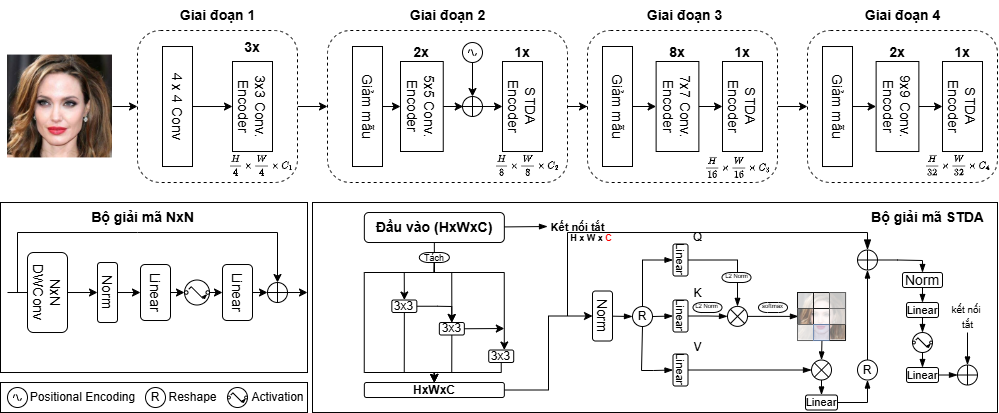
\includegraphics[width=0.9\textwidth]{images/edgeNext.png}
    \caption{Kiến trúc tổng thể của EdgeNext .}
    \label{fig:edgenext_architecture}
\end{figure}

\begin{verbatim}
Input Image (3 × 224 × 224)
     ↓
[Stem]: Conv 4×4, stride 4 → (C1 × 56 × 56)
     ↓
Stage 1: 3 × Conv Encoder (kernel 3×3)
     ↓
Stage 2: Downsample (2×2) + 2 × Conv Encoder (5×5) + 1 × SDTA Encoder + Positional Encoding
     ↓
Stage 3: Downsample + 8 × Conv Encoder (7×7) + 1 × SDTA Encoder
     ↓
Stage 4: Downsample + 2 × Conv Encoder (9×9) + 1 × SDTA Encoder
     ↓
Global Average Pooling → Classifier
\end{verbatim}

\begin{itemize}
    \item \textbf{Stem}: Sử dụng một lớp convolution 4×4 (stride 4) không chồng lấp để giảm kích thước không gian nhanh chóng, sau đó áp dụng \textbf{Layer Normalization (LN)} thay vì BatchNorm để ổn định huấn luyện.
    \item \textbf{Conv Encoder}: Mỗi block bao gồm:
    \begin{itemize}
        \item Depth-wise convolution (kernel thích ứng)
        \item Hai point-wise convolution (1×1)
        \item LayerNorm + GELU + Skip connection
    \end{itemize}
    \textrightarrow Công thức:
    \[
    x_{out} = x_{in} + \text{Linear}_2(\text{GELU}(\text{Linear}_1(\text{LN}(\text{DwConv}(x_{in})))))
    \]
    \item \textbf{SDTA Encoder}: Kết hợp depth-wise conv 3×3 và transpose attention theo chiều kênh. \\
    \textrightarrow Công thức attention:
    \[
    \text{Attention}(Q, K, V) = V \cdot \text{softmax}\left(\frac{Q^T K}{\sqrt{d}}\right)
    \]
    với $Q, K, V \in \mathbb{R}^{C \times N}$, $d$ là chiều ẩn.
    \item \textbf{Positional Encoding}: Chỉ được thêm vào \textbf{trước block SDTA ở Stage 2} để cung cấp thông tin vị trí mà không làm tăng độ trễ ở các giai đoạn sau.
\end{itemize}

\textbf{Tóm lại}, EdgeNext là một bước tiến trong việc thiết kế mô hình thị giác tinh gọn, kết hợp hiệu quả giữa \textbf{tính cục bộ của CNN} và \textbf{tính toàn cục của Transformer} thông qua các cải tiến về attention tuyến tính và convolution đa tỷ lệ. Những nguyên tắc này không chỉ giúp mô hình hoạt động tốt trên thiết bị biên mà còn tạo nền tảng vững chắc cho các ứng dụng chuyên biệt như \textbf{nhận diện khuôn mặt} -- sẽ được phát triển thành \textbf{EdgeFace} trong phần tiếp theo.
% Giới thiệu tổng quan về edgeface
%% Trình bày EdgeFce là mô hình nhận diện khuôn mặt nhẹ, thiết kế cho thiết bị biên
%% Nêu rõ mục tiêu tối ưu hóa hiệu quả tính toán và lưu trữ

% Thích nghi cho nhận diện khuôn mặt
%% Mô tả Edgeface dựa trên kiến trúc Edgenext, với các lớp linear được thay bằng Low Rank Linear(loRaLin) để giảm tham số và FLOPs.
%% Đề cập điều chỉnh độ phân giải đầu vào thành 112x112 cho phù hợp với nhận diện khuôn mặt


% Classification Head 
%% giới thiệu classification Head gồm : Adaptive Average Pooling, LayerNorm, LoRaLin layer(tạo embedding 512 chiều)

%Minh họa kiến trúc 
%% Nhắc đến hình 1 trong bài báo gốc [George et al., 2024], minh họa sơ đồ kiến trúc EdgeFace, bao gồm các stage với bộ mã hóa 


% Kết luận ngắn gọn 
%% Tóm tắt EdgeFace là mô hình hiệu quả, sử dụng LoRaLin và classification head để tạo embedding chất lượng cao 



\subsection{Kiến trúc EdgeNeXt}

EdgeNeXt là một kiến trúc thị giác lai (\textit{hybrid architecture}) kết hợp giữa \textbf{Convolutional Neural Network (CNN)} và \textbf{Transformer}. Mục tiêu của EdgeNeXt là khai thác điểm mạnh của cả hai hướng tiếp cận: CNN hiệu quả trong việc trích xuất đặc trưng cục bộ, trong khi Transformer có khả năng mô hình hóa ngữ cảnh toàn cục. Bằng cách kết hợp, EdgeNeXt vừa giữ được độ chính xác cao, vừa duy trì chi phí tính toán thấp, phù hợp để triển khai trên \textit{thiết bị biên}. 

Khác với ConvNeXt – mô hình gốc mà EdgeNeXt phát triển từ đó – EdgeNeXt được thiết kế lại với các cơ chế tính toán nhẹ hơn, nhằm giảm số tham số và phép nhân-cộng (MAdds), đồng thời vẫn đảm bảo hiệu quả trên các tác vụ thị giác máy tính quy mô lớn.

\subsubsection{Bộ mã hóa Split Depth-wise Transpose Attention (SDTA)}
Trọng tâm đổi mới của EdgeNeXt nằm ở \textbf{SDTA encoder}, một khối mã hóa đặc trưng gọn nhẹ nhưng mạnh mẽ. Cơ chế của SDTA bao gồm:
\begin{itemize}
    \item \textbf{Phân chia nhóm kênh}: tensor đầu vào được tách thành nhiều nhóm kênh để xử lý song song, giúp giảm tải tính toán.
    \item \textbf{Depth-wise convolution}: áp dụng tích chập theo từng kênh để nắm bắt thông tin cục bộ với chi phí rẻ.
    \item \textbf{Self-attention dạng hoán vị}: sử dụng truy vấn (query) và khóa (key) được hoán vị theo chiều kênh, cho phép tính toán attention với độ phức tạp tuyến tính thay vì bậc hai.
\end{itemize}

Nhờ thiết kế này, SDTA mở rộng được \textit{trường tiếp nhận} (receptive field) mà không cần tăng nhiều tham số. Kết quả là mô hình có thể biểu diễn đặc trưng đa tỷ lệ (\textit{multi-scale features}), rất quan trọng cho các tác vụ nhận diện và phân loại ảnh.

\subsubsection{Kernel thích ứng}
Để tăng cường khả năng mô hình hóa thông tin toàn cục, EdgeNeXt sử dụng \textbf{kernel tích chập thích ứng} qua từng giai đoạn (stage). Cụ thể, các lớp đầu thường sử dụng kernel nhỏ (ví dụ: $3 \times 3$) nhằm tập trung vào chi tiết cục bộ, trong khi các lớp sâu hơn chuyển sang kernel lớn hơn (ví dụ: $9 \times 9$) để khai thác thông tin toàn ảnh. Cách tiếp cận này cho phép mô hình dần dần tích hợp ngữ cảnh rộng hơn mà không làm chi phí tính toán tăng đột biến.

\subsubsection{Các biến thể của EdgeNeXt}
Để đáp ứng đa dạng yêu cầu tài nguyên, EdgeNeXt được triển khai dưới nhiều biến thể: \textbf{Small}, \textbf{X-Small} và \textbf{XX-Small}. Các phiên bản này khác nhau về độ sâu mạng, số kênh đặc trưng và tổng tham số, từ đó cho phép người dùng cân nhắc giữa độ chính xác và chi phí tính toán. Bảng~1 trong bài báo gốc~\cite{george2024edgeface} minh họa chi tiết cấu trúc lớp, số kênh và đầu ra của từng biến thể, cung cấp sự linh hoạt cao trong triển khai thực tế.

\subsubsection{Hiệu suất và minh họa}
Theo các thực nghiệm trong~\cite{george2024edgeface}, EdgeNeXt đạt hiệu suất vượt trội so với nhiều mô hình lightweight khác như MobileViT hay EdgeFormer, đặc biệt trong tác vụ phân loại ảnh. Ưu điểm nổi bật là đạt độ chính xác tương đương hoặc cao hơn trong khi chi phí tính toán thấp hơn đáng kể. Ngoài ra, sơ đồ cấu trúc và thông số minh họa ở Bảng~1 cung cấp cái nhìn trực quan về cách EdgeNeXt đạt được sự cân bằng giữa độ chính xác và hiệu quả tính toán.\\



\begin{table}[ht]
  \caption{So sánh các mô hình lightweight: EdgeNeXt, MobileViT, EdgeFormer, EdgeFace(Số liệu ảo)}
  \label{tab:compare_lightweight}
  \centering
  \begin{tabularx}{\textwidth}{l c c p{3cm} p{3.2cm}}
    \toprule
    \textbf{Mô hình} & \textbf{Tham số} & \textbf{MAdds} & \textbf{Độ chính xác} & \textbf{Ghi chú} \\
    \midrule
    EdgeNeXt (Small) & $\sim$1.3M & thấp & Top-1 $\approx$ 71.2\% (ImageNet) & Giảm FLOPs $\sim$28\% so với MobileViT \\
    MobileViT & — & — & — & Đối thủ lightweight CNN–Transformer \\
    EdgeFormer & — & — & — & Mô hình lai lightweight, dùng cho biên \\
    EdgeFace & $\sim$1.77M & — & LFW 99.73\%; IJB-B 92.67\%; IJB-C 94.85\% & Tối ưu dưới 2M tham số, dùng LoRaLin \\
    \bottomrule
  \end{tabularx}
\end{table} 


Tóm lại, EdgeNeXt là một kiến trúc lai kết hợp CNN và Transformer, trong đó SDTA encoder và kernel thích ứng đóng vai trò trung tâm. Nhờ thiết kế này, EdgeNeXt đạt được sự cân bằng giữa khả năng biểu diễn và chi phí tính toán, trở thành lựa chọn phù hợp cho các ứng dụng thị giác trên thiết bị biên.

%Mở đầu: Giới thiệu tổng quan về EdgeNeXt

%%Trình bày EdgeNeXt là một kiến trúc hybrid kết hợp CNN và Transformer, được thiết kế để tối ưu cho thiết bị biên với số lượng tham số và phép tính (MAdds) thấp.
%%Nêu rõ EdgeNeXt phát triển dựa trên ConvNeXt, cải tiến để phù hợp cho các ứng dụng thị giác máy tính.

%Split Depth-wise Transpose Attention (SDTA) Encoder

%%Mô tả SDTA là thành phần cốt lõi, phân chia tensor đầu vào thành các nhóm kênh.
%%Giải thích cơ chế: Sử dụng depth-wise convolution kết hợp self-attention theo chiều kênh (transposed query-key) để đạt độ phức tạp tuyến tính.
%%Nêu vai trò của SDTA: Mở rộng trường tiếp nhận (receptive field) và mã hóa đặc trưng đa tỷ lệ (multi-scale).

%Kernel thích ứng

%%Mô tả việc sử dụng kernel kích thước khác nhau qua các stage (3x3 ở lớp đầu, lớn hơn như 9x9 ở lớp sau) để thu thập thông tin toàn cục.
%%Đề cập rằng kernel thích ứng giúp tăng cường khả năng mã hóa đặc trưng toàn cục.

%Các biến thể của EdgeNeXt

%%Giới thiệu các biến thể: Small, X-Small, XX-Small, với kích thước đặc trưng và tham số khác nhau (tham khảo Table 1 trong bài báo gốc [George et al., 2024]).
%%Nêu rõ các biến thể cung cấp tính linh hoạt tùy thuộc vào yêu cầu tài nguyên.

%Hiệu suất và minh họa

%%Nhắc đến hiệu suất của EdgeNeXt: Vượt trội so với MobileViT và EdgeFormer trong nhận diện hình ảnh với chi phí tính toán thấp.
%%Đề cập Table 1 minh họa cấu trúc lớp, kích thước đầu ra, và số kênh cho các biến thể.

%Kết luận ngắn gọn

%%Tóm tắt rằng EdgeNeXt kết hợp CNN và Transformer với SDTA và kernel thích ứng, cung cấp kiến trúc hiệu quả cho các ứng dụng trên thiết bị biên.

\subsection{Mô-đun tuyến tính hạng thấp(LoRaLin)}

 
Trong các kiến trúc học sâu, đặc biệt là trong các mô hình nhận diện khuôn mặt, các lớp tuyến tính (\textit{fully connected layers}) thường chiếm một tỷ lệ lớn số tham số và chi phí tính toán. Để giải quyết thách thức này trong bối cảnh triển khai trên thiết bị biên, EdgeFace giới thiệu \textbf{Low Rank Linear Module (LoRaLin)} như một cải tiến quan trọng. Mục tiêu của LoRaLin là giảm đáng kể số lượng tham số và phép tính (\textit{Multiply-Adds, MAdds}) trong khi chỉ làm suy giảm hiệu suất ở mức tối thiểu.

\paragraph{Cơ chế phân tích low-rank.} 
Ý tưởng cốt lõi của LoRaLin là phân tích ma trận trọng số full-rank thành hai ma trận hạng thấp. Cho một lớp tuyến tính chuẩn với ma trận trọng số $W \in \mathbb{R}^{M \times N}$, LoRaLin thay thế bằng tích của hai ma trận nhỏ hơn:
\[
    W_{M \times N} \approx W_{M \times r} \cdot W_{r \times N},
\]
trong đó $r$ là \textit{rank} được xác định theo công thức:
\[
    r = \max(2, \gamma \cdot \min(M,N)),
\]
với $\gamma$ là tham số \textit{rank-ratio}. Cách tiếp cận này tương đương với việc thay thế một lớp tuyến tính duy nhất bằng hai lớp tuyến tính liên tiếp: lớp thứ nhất giảm chiều xuống $r$, và lớp thứ hai ánh xạ trở lại không gian đầu ra. Hình~2 trong bài báo gốc~\cite{george2024edgeface} minh họa trực quan cơ chế này.\\



\paragraph{Điều chỉnh Rank-ratio ($\gamma$).} 
Tham số $\gamma$ quyết định mức độ giảm hạng và do đó ảnh hưởng trực tiếp đến số tham số và FLOPs. Kết quả thực nghiệm (Hình~3 trong~\cite{george2024edgeface}) cho thấy:
\begin{figure}[ht]
    \centering
    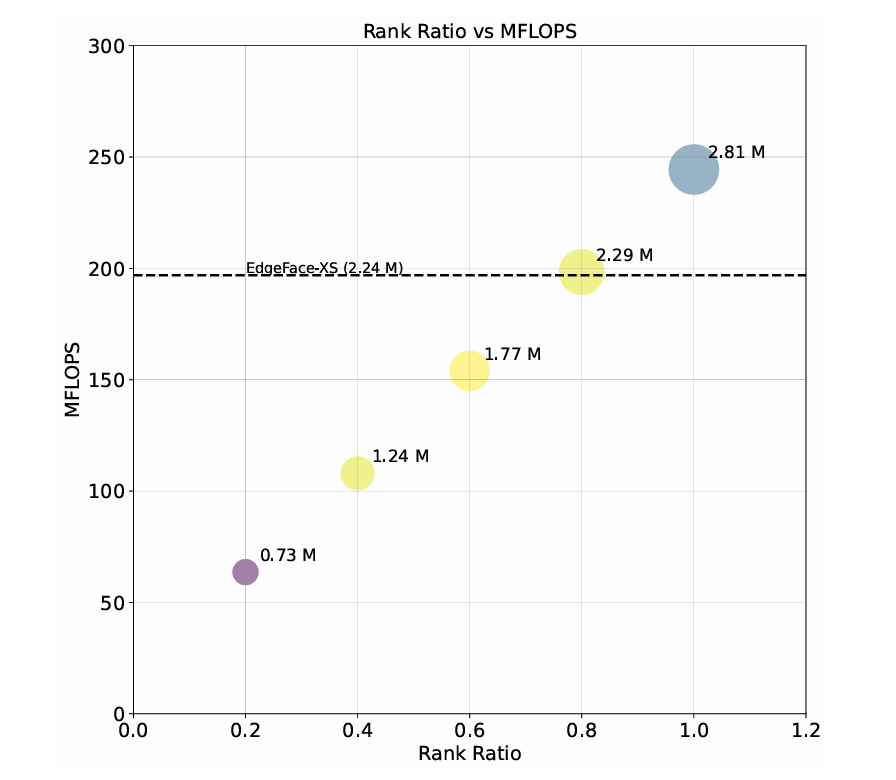
\includegraphics[width=0.65\textwidth]{images/fig3.2.3.png} % đường dẫn 
    \caption{Ảnh hưởng của tham số \textit{Rank-ratio} ($\gamma$) đến số lượng tham số của mô hình (MPARAMS) và số phép nhân-cộng (MFLOPs). 
    Đường nét đứt thể hiện giá trị tham chiếu của mô hình gốc khi sử dụng lớp tuyến tính thông thường. 
    Có thể thấy khi $\gamma$ giảm, số tham số và FLOPs giảm đáng kể, trong khi vẫn duy trì hiệu suất gần như không đổi.}
    \label{fig:lora_lin_rank}
    
\end{figure}

\begin{itemize}
    \item Khi $\gamma < 0.8$, số tham số và FLOPs giảm đáng kể so với lớp tuyến tính chuẩn.
    \item Ở $\gamma \approx 0.6$, EdgeFace đạt \textbf{sự cân bằng tối ưu}: giảm khoảng $20\%$ số tham số và FLOPs, trong khi suy giảm hiệu suất dưới $0.5\%$.
\end{itemize}
Điều này chứng tỏ LoRaLin mang lại khả năng nén mô hình hiệu quả với trade-off tối thiểu về độ chính xác.

\paragraph{Triển khai và minh họa.} 
Trong PyTorch, LoRaLin có thể được triển khai đơn giản bằng cách xâu chuỗi hai lớp tuyến tính:
\begin{itemize}
    \item \texttt{lin1}: ánh xạ từ \texttt{in\_feat} $\to$ \texttt{rank}.
    \item \texttt{lin2}: ánh xạ từ \texttt{rank} $\to$ \texttt{out\_feat}.
\end{itemize}
Nhờ thiết kế này, LoRaLin có thể thay thế trực tiếp các lớp tuyến tính truyền thống trong EdgeFace mà không làm phức tạp thêm quá trình huấn luyện hay suy luận. Trên thực tế, toàn bộ các lớp fully connected trong EdgeFace đều được thay bằng LoRaLin để tối ưu hiệu quả tính toán.

\paragraph{Kết luận.} 
Tóm lại, \textbf{LoRaLin} là một giải pháp gọn nhẹ và hiệu quả để giảm số tham số và FLOPs trong các lớp fully connected. Với cơ chế phân tích hạng thấp và khả năng điều chỉnh linh hoạt qua $\gamma$, LoRaLin cho phép EdgeFace duy trì chất lượng biểu diễn embedding gần như không suy giảm, đồng thời đáp ứng yêu cầu triển khai trên thiết bị biên.

\subsection{Chi tiết huấn luyện}
\subsubsection{Chiến lược huấn luyện}

EdgeFace được huấn luyện nhằm tối ưu hóa hiệu suất nhận diện khuôn mặt trong điều kiện hạn chế tài nguyên trên thiết bị biên. 
Quy trình huấn luyện tận dụng tập dữ liệu quy mô lớn kết hợp với các chiến lược tối ưu hóa để vừa nâng cao độ chính xác, vừa duy trì tính gọn nhẹ của mô hình \cite{george2024edgeface}.

\textbf{Dataset.} Mô hình được huấn luyện trên các tập con WebFace12M và WebFace4M, được trích xuất từ WebFace260M. 
Các ảnh trong tập dữ liệu này đã được căn chỉnh khuôn mặt và chuẩn hóa độ phân giải về $112\times112$, phù hợp với tiêu chuẩn của các hệ thống nhận diện khuôn mặt.

\textbf{Tiền xử lý và tăng cường dữ liệu.} Dữ liệu đầu vào được chuyển đổi thành tensor và chuẩn hóa về khoảng $[-1,1]$. 
Quá trình tăng cường dữ liệu được thực hiện bằng thư viện DALI, bao gồm các phép biến đổi như chuyển đổi ngẫu nhiên sang thang xám, thay đổi kích thước, và làm mờ, nhằm tăng tính đa dạng và tính khái quát của mô hình.

\textbf{Chi tiết huấn luyện.} Mô hình được huấn luyện trên 4--8 GPU Nvidia RTX 3090 (24GB) với chiến lược \textit{distributed training}. 
Optimizer AdamW kết hợp với hàm mất mát CosFace được sử dụng để tối ưu embedding. 
Lịch trình learning rate theo \textit{polynomial decay with restarts} giúp mô hình hội tụ ổn định. 
Batch size dao động từ 256 đến 512 tùy thuộc vào kích thước mô hình, và PartialFC được áp dụng để xử lý số lượng lớn danh tính trong tập dữ liệu.

\textbf{Inference.} Trong giai đoạn suy luận, \textit{classification head} được loại bỏ. 
Mô hình chỉ sử dụng vector embedding 512 chiều làm biểu diễn đặc trưng cho so sánh và truy hồi khuôn mặt.

Tóm lại, quy trình huấn luyện của EdgeFace kết hợp dữ liệu quy mô lớn, tiền xử lý hiệu quả, và các kỹ thuật tối ưu hóa hiện đại, từ đó đạt được hiệu suất cao trong khi vẫn đảm bảo khả năng triển khai trên thiết bị biên.
